\begin{frame}{Scientific context}
    \textbf{Context :} Create real-time digital twins of an organ, described by a levelset function.
    
    $\rightarrow$ This levelset function can easily be obtained from medical images.

    \textbf{$\phi$-FEM Method :} New fictitious domain finite element method.

    \begin{itemize}[\ding{217}]
        \item domain given by a level-set function $\Rightarrow$ don't require a mesh fitting the boundary 
        \item allow to work on complex geometries 
        \item ensure geometric quality of the mesh
        % \item Cartesian grid adapted for neural networks
    \end{itemize}
    
    \begin{center}
        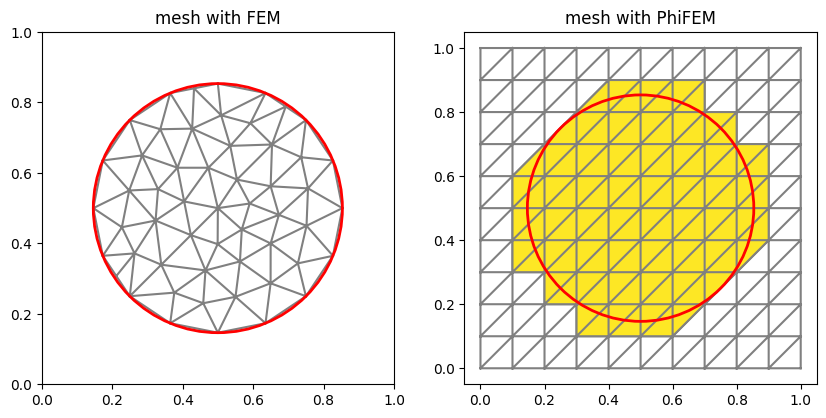
\includegraphics[width=0.55\linewidth]{images/intro/context_geometry.png}
    \end{center}	

    \textit{Practical cases:} Real-time simulation, shape optimization...
    
    \textbf{Neural Network :} Obtain a solution quickly.
\end{frame}

\begin{frame}{Problem considered}
    \textbf{Elliptic problem with Dirichlet conditions :} \\
    Find $u : \Omega \rightarrow \mathbb{R}^d (d=1,2,3)$ such that
    \begin{equation}
    	\left\{\begin{aligned}
    		&L(u)=-\nabla \cdot (A(x) \nabla u(x)) + c(x)u(x) = f(x) \quad \text{in } \Omega, \\
    		&u(x) = g(x) \quad \text{on } \partial \Omega
    	\end{aligned}\right. \label{edp}
    \end{equation}
	with $A$ a definite positive coercivity condition and $c$ a scalar. We consider $\Delta$ the Laplace operator, $\Omega$ a smooth bounded open set and $\Gamma$ its boundary. 
	
    \textbf{Weak formulation :}
    \begin{equation*}
    	\text{Find } u\in V \text{ such that } a(u, v) = l (v) \forall v\in V
    \end{equation*}
    
    with
    \begin{align*}
    	a(u,v)&=\int_{\Omega} (A(x)\nabla u(x)) \cdot \nabla v(x) + c(x)u(x)v(x) \, dx \\
    	l(v)&=\int_{\Omega} f(x)v(x) \, dx
    \end{align*}
\end{frame}

\begin{frame}{Aim of the talk}
	\textbf{Objective :} Show that the philosophy behind most of the methods is the same.
	\begin{center}
		Mesh-based methods \hspace{5pt} // \hspace{5pt} Physically informed learning
	\end{center}
	
	\textbf{Numerical methods :} Discretize an infinite-dimensional problem (unknown = function) and solve it in a finite-dimensional space (unknown = vector).
	\begin{itemize}[\textbullet]
		\item \textbf{Encoding :} we encode the problem in a finite-dimensional space
		\item \textbf{Approximation :} solve the problem in finite-dimensional space
		\item \textbf{Decoding :} bring the solution back into infinite dimensional space
	\end{itemize}
	
	\begin{center}
		\begin{tabular}{|c|c|c|}
			\hline
			\textbf{Encoding} & \textbf{Approximation} & \textbf{Decoding} \\
			\hline
			$f \; \rightarrow \theta_f$ & $\theta_f \; \rightarrow \theta_u$ & $\theta_u \; \rightarrow u_\theta$ \\
			\hline
		\end{tabular}
	\end{center}

	\bigskip

	\textbf{Projector :} Encoder + Decoder
	\begin{figure}[htb]
		\vspace{-10pt}
		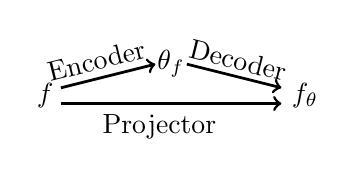
\begin{tikzpicture}
			\node at (-0.2,0) {$f$};
			\draw[->, line width=1pt] (0,0.1) -- (1.2,0.4);
			\node at (1.4,0.4) {$\theta_f$};
			\draw[->, line width=1pt] (1.6,0.4) -- (2.8,0.1);
			\node at (3.1,0) {$f_\theta$};
			\draw[->, line width=1pt] (0,-0.1) -- (2.8,-0.1);
			
			\node[rotate=14] at (0.45,0.45) {Encoder};
			\node[rotate=-14] at (2.25,0.45) {Decoder};
			\node at (1.25,-0.4) {Projector};
		\end{tikzpicture} 
	\end{figure}
\end{frame}
